%%%%%%%%%%%%%%%%%%%%%%%%%%%%%%%%%%%%%%%%%%%%%%%%%%%%%%%%%%%%%%%%%%%%%%
% Skupina01/main.tex -- VZOREC POGLAVJA
%
% Ta datoteka je primer, kako je poglavje zgrajeno. Kopirajte jo v svoj
% direktorij SkupinaXX, zamenjajte "g01:" z "gXX:" in besedilo v oglatih
% oklepajih [ ... ] nadomestite s svojim.
%
% Pravila:
%  - brez \usepackage (vse pakete naloži editor.tex),
%  - slike v SkupinaXX/img/, vse oznake in ključi virov z "gXX:",
%  - vire dodajte v skupno datoteko references.bib (z doi ali url).
%%%%%%%%%%%%%%%%%%%%%%%%%%%%%%%%%%%%%%%%%%%%%%%%%%%%%%%%%%%%%%%%%%%%%%
\graphicspath{{Skupina27/img/}}

\title{Analiza odpornosti QCA demultiplekserja na napake zaradi premikov celic}
% \titlerunning{[Krajši naslov]}  % če je naslov predolg za glavo strani
\author{Vojko Hysz, Gašper Suhadolnik in Matic Poženel}
\maketitle

% \abstract{[Povzetek v 5 do 10 vrsticah. Navedite raziskovalno vprašanje, uporabljeno metodo in orodja ter glavni rezultat s konkretno številko, npr.\ \enquote{Fizično reverzibilna izvedba polnega seštevalnika potrebuje 2,3-krat več celic in ima 1,5 urina cikla večjo zakasnitev kot ireverzibilna, disipira pa 40~\% manj energije.} Končajte z enim stavkom o pomenu rezultata.]}

\abstract{V seminarski nalogi smo podrobneje analizirali 27-celično implementacijo demultiplekserja $1:2$, ki je zasnovan v tehnologiji kvantnih celičnih avtomatov (QCA). Preverjali smo vpliv premikov celic v ključnih komponentah in v bližini vhodov in izhodov ter podrobno analizirali pravilnost delovanja in polarizacijo izhodov pri posameznih premikih vsake celice. Eksperimenti so pokazali, da celice v majoritetnih vratih povrzočijo nepravilno delovanje pri premiku za 1nm, medtem ko celica v negatorju ne povzroči napake niti ob premiku za 5nm. Raziskava potrjuje, da so položaj in smer odstopanja posamezne celice pomembni dejavniki pri zanesljivosti delovanja QCA-vezij.}


% \begin{abstract}
% V seminarski nalogi smo preučevali vpliv fizičnih premikov posameznih celic na delovanje demultiplekserja $1:2$, zasnovanega s tehnologijo kvantnih celičnih avtomatov (QCA). Izhajali smo iz 27-celične implementacije, predstavljene v literaturi, in jo rekonstruirali v programskem orodju QCADesigner-E. Posamezne celice na različnih mestih vezja smo premikali za 1, 3 in 5 nm v različnih smereh ter analizirali vpliv teh sprememb na pravilnost izhodov, toleranco na premike in izhodno polarizacijo. Rezultati so pokazali, da občutljivost vezja ni enakomerno porazdeljena. Najbolj občutljive so bile celice v območju majoritetnih vrat 0, predvsem M0a in M0c, ter celica W2 na vhodnem povezovalnem vodilu. Nasprotno je negator ohranil pravilno delovanje pri vseh preizkušenih premikih. Ugotovili smo tudi, da na izhodno polarizacijo najbolj vplivajo premiki celic, ki neposredno mejijo na izhode. Z večanjem premikov se je povečeval tudi delež neuspešnih simulacij. Raziskava potrjuje, da so položaj in smer odstopanja posamezne celice pomembni dejavniki pri zanesljivosti delovanja QCA-vezij.

% \textbf{Ključne besede:} kvantni celični avtomati, QCA, demultiplekser, QCADesigner-E, premik celic, polarizacija, zanesljivost.
% \end{abstract}



\section{Uvod}
\label{g27:sec:uvod}

Zaradi nenehnega razvoja računalniške tehnologije in vse večjih zahtev po zmogljivosti elektronskih naprav se pojavlja potreba po novih načinih implementacije logičnih vezij. Klasična tehnologija CMOS (angl. \textit{Complementary Metal-Oxide-Semiconductor}), ki temelji na uporabi tranzistorjev, se pri nadaljnjem zmanjševanju dimenzij sooča z različnimi fizikalnimi omejitvami. Med pomembnejše težave sodijo uhajalni tokovi, segrevanje in vse večja poraba energije. Kot ena izmed možnih alternativ se je razvila tehnologija kvantnih celičnih avtomatov (QCA, angl. \textit{Quantum-dot Cellular Automata}), ki so jo leta 1993 predstavili Lent in sodelavci \cite{lent1993}.

\subsection{Kvantni celični avtomati}

Tehnologija QCA predstavlja drugačen pristop k načrtovanju digitalnih vezij, saj za prenos in obdelavo informacij ne uporablja klasičnega električnega toka skozi tranzistorje, temveč elektrostatične interakcije med sosednjimi celicami. Osnovni gradnik te tehnologije je kvantna celica, ki je sestavljena iz štirih kvantnih pik, razporejenih na ogliščih kvadrata. V celici sta dva elektrona, ki se zaradi medsebojnega elektrostatičnega odboja razporedita v nasprotni oglišči. Tako nastaneta dve stabilni konfiguraciji, ki predstavljata logični stanji 0 in 1. Stanje celice opišemo s polarizacijo $P$, pri čemer vrednost $P=-1$ predstavlja logično 0, vrednost $P=+1$ pa logično 1.

Informacija se med sosednjimi celicami prenaša preko elektrostatičnega vpliva, pri čemer polarizacija ene celice vpliva na polarizacijo sosednjih celic. S povezovanjem več celic lahko tako ustvarimo logična vrata, povezovalna vodila in kompleksnejša digitalna vezja. Pomembna prednost tehnologije QCA je možnost zelo majhnih dimenzij vezij, visoke gostote integracije in potencialno nizke porabe energije, saj za delovanje ni potreben običajen električni tok skozi logične elemente. Poleg tega lahko QCA omogoča zelo hitro obdelavo informacij na nanometrski ravni \cite{lent1993}.

Kljub omenjenim prednostim ima tehnologija QCA tudi nekatere pomembne omejitve. Delovanje celic je močno odvisno od njihovih medsebojnih elektrostatičnih interakcij, zato lahko že manjša odstopanja pri njihovi izdelavi vplivajo na pravilnost prenosa informacij. Med možne napake sodijo manjkajoče celice, napačna orientacija celic in njihovi fizični premiki glede na predvideno lego. Sprememba razdalje med celicami namreč vpliva na moč medsebojnega elektrostatičnega vpliva in posledično na njihovo polarizacijo. Dodatne omejitve predstavljajo temperaturna občutljivost, zahteve glede natančnosti izdelave ter potreba po ustreznem uravnavanju urnih signalov. Zaradi teh lastnosti je zanesljivost delovanja QCA-vezij pomembno področje raziskav \cite{khan2023}.

\subsection{Demultiplekser 1:2}

Demultiplekser je kombinacijsko logično vezje, ki en vhodni podatkovni signal usmerja na enega izmed več izhodov. Izbira izhoda je določena z vrednostjo izbirnih oziroma krmilnih vhodov. Demultiplekser $1:2$ ima en podatkovni vhod $D$, en izbirni vhod $S$ in dva izhoda $Y_0$ ter $Y_1$. Glede na vrednost izbirnega vhoda se vhodni signal prenese na ustrezni izhod, medtem ko drugi izhod ostane v logičnem stanju 0.

Logično delovanje demultiplekserja $1:2$ lahko opišemo z naslednjima enačbama:

\begin{equation}
Y_0 = D \cdot \overline{S}
\end{equation}

\begin{equation}
Y_1 = D \cdot S
\end{equation}

Iz enačb je razvidno, da se vhodni signal $D$ prenese na izhod $Y_0$, kadar je $S=0$, oziroma na izhod $Y_1$, kadar je $S=1$. Če je vhodni signal $D=0$, sta oba izhoda ne glede na vrednost izbirnega vhoda enaka 0. Delovanje vezja prikazuje tabela~\ref{tab:demux}.

\begin{table}[h]
\centering
\caption{Resničnostna tabela demultiplekserja $1:2$.}
\label{tab:demux}
\begin{tabular}{c|c|c|c}
$D$ & $S$ & $Y_0$ & $Y_1$ \\
\hline
0 & 0 & 0 & 0 \\
0 & 1 & 0 & 0 \\
1 & 0 & 1 & 0 \\
1 & 1 & 0 & 1 \\
\end{tabular}
\end{table}

Demultiplekserji se uporabljajo predvsem za usmerjanje podatkov in porazdeljevanje signalov v digitalnih sistemih. Najdemo jih v komunikacijskih sistemih, kjer omogočajo razdeljevanje sprejetih podatkovnih signalov, ter v mikroprocesorskih sistemih, pomnilniških vezjih in digitalnih krmilnih enotah. Večje demultiplekserje, na primer $1:4$ in $1:8$, lahko sestavimo z zaporednim povezovanjem manjših demultiplekserjev $1:2$.

\subsection{Logična vrata v tehnologiji QCA}

Pri načrtovanju logičnih vezij QCA sta posebej pomembna dva gradnika: majoritetna vrata in negator. Trivhodna majoritetna vrata (angl. \textit{Majority Gate}) imajo tri vhode $A$, $B$ in $C$ ter en izhod $M$. Izhodna vrednost je določena z večinskim stanjem vhodov. Njihovo logično funkcijo opišemo z izrazom:

\begin{equation}
M(A,B,C)=AB+AC+BC.
\end{equation}

Izhod je torej enak 1, če sta vsaj dva izmed treh vhodov enaka 1, sicer je enak 0. Z ustrezno nastavitvijo enega izmed vhodov lahko majoritetna vrata uporabimo tudi kot AND oziroma OR vrata. Če je na primer vhod $C$ nastavljen na 0, dobimo funkcijo AND, če pa je nastavljen na 1, dobimo funkcijo OR.

Drugi pomemben gradnik je negator oziroma invertor (NOT), ki obrne logično vrednost vhodnega signala. V QCA se lahko realizira z ustrezno razporeditvijo celic, pri kateri zaradi njihove medsebojne elektrostatične interakcije na izhodu dobimo nasprotno polarizacijo od vhodne. Kombinacija majoritetnih vrat in negatorjev omogoča realizacijo različnih kombinacijskih logičnih vezij, med katere spada tudi demultiplekser.

\subsection{Implementacija demultiplekserja 1:2 v QCA}

Demultiplekser $1:2$ lahko v tehnologiji QCA realiziramo z uporabo enega negatorja in dveh majoritetnih vrat. Majoritetna vrata lahko s primerno nastavitvijo tretjega vhoda uporabimo kot AND vrata. Prva vrata tako izračunajo izraz $D\overline{S}$, druga pa $DS$. Za pravilno delovanje vezja je pomembna tudi ustrezna razporeditev celic, saj ta določa prenos polarizacije med logičnimi elementi.

V literaturi je bilo predstavljenih več različnih implementacij demultiplekserja $1:2$. Razlikujejo se predvsem po številu uporabljenih celic, velikosti vezja, zakasnitvi, energijski disipaciji in načinu povezovanja posameznih logičnih elementov. Nekatere zasnove uporabljajo manjše število celic in dosegajo krajšo zakasnitev, vendar imajo lahko težave pri povezovanju z drugimi vezji, dostopnosti vhodnih in izhodnih celic ali zanesljivosti prenosa polarizacije. Druge zasnove dajejo prednost enostavnejšemu povezovanju in modularnosti, vendar za to potrebujejo več celic in večjo površino.

V izhodiščnem članku Paramjeet in sod. \cite{paramjeet2026} je predstavljena modularna implementacija demultiplekserja $1:2$, ki uporablja 27 QCA-celic. Vezje je zasnovano v eni ravnini (angl. \textit{coplanar design}) in omogoča neposreden dostop do vseh vhodov in izhodov, kar poenostavlja povezovanje več enakih modulov v kompleksnejša vezja. Avtorji so predlagano zasnovo simulirali v programu QCADesigner 2.0.3, energijsko disipacijo pa analizirali z razširitvijo QCADesigner-E. Rezultati kažejo, da vezje pravilno opravlja funkcijo demultiplekserja, pri čemer znaša njegova zakasnitev en urini cikel. Predlagana zasnova predstavlja osnovni gradnik za modularno sestavljanje večjih demultiplekserjev, kot sta $1:4$ in $1:8$ \cite{paramjeet2026}. Shemo implementacije prikazuje slika \ref{g27:fig:shema-27}.


\begin{figure}[htbp]
    \centering
    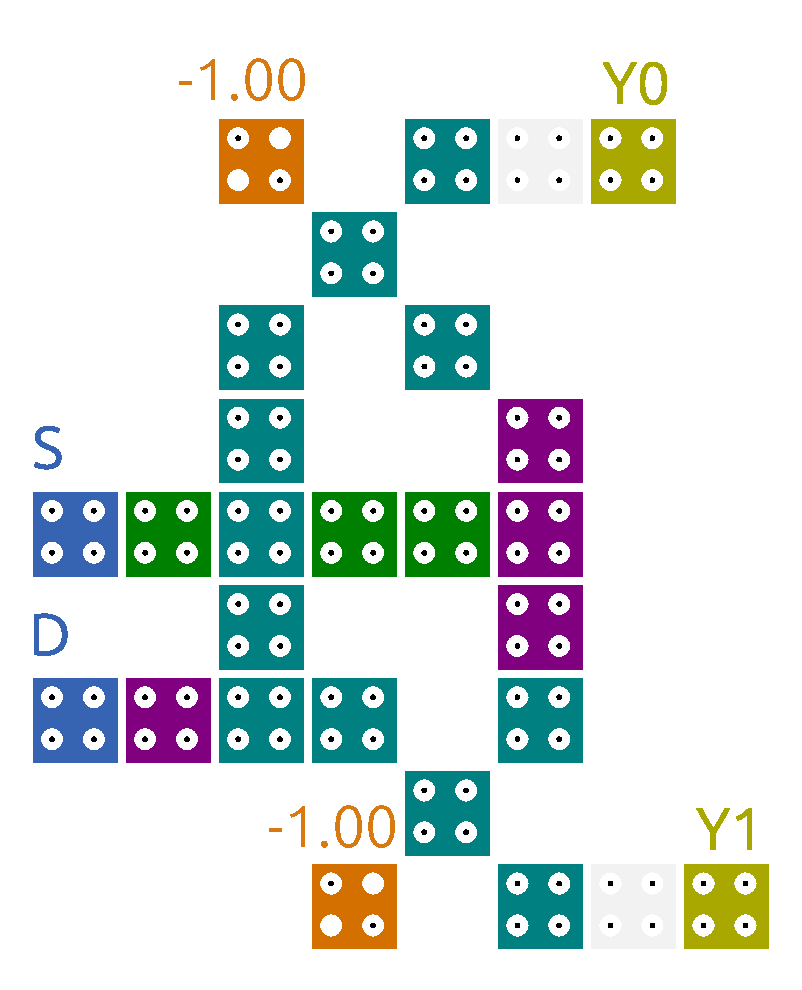
\includegraphics[width=0.5\textwidth]{demux27.pdf}
    \caption{
        Shema implementacije demultiplekserja s 27 celicami. Celici z oznakama s in d sta vhodni, celici z oznakama y0 in y1 pa izhodni. Celici z oranžno barvo sta s fiksiranim stanjem.
    }
    \label{g27:fig:shema-27}
\end{figure}

Kljub uspešnemu preverjanju funkcionalnosti pa ostaja pomembno vprašanje odpornosti takšnih vezij na fizične nepravilnosti. Ker delovanje QCA temelji na elektrostatičnih interakcijah med celicami, lahko spremembe njihovih položajev vplivajo na polarizacijo in s tem na pravilnost delovanja logičnih vrat. Zato je smiselno raziskati, kako občutljive so posamezne celice na premike ter ali so celice v območju logičnih vrat bolj občutljive od tistih v povezovalnih vodilih. Takšna analiza lahko prispeva k boljšemu razumevanju zanesljivosti QCA-vezij in njihovih omejitev pri praktični implementaciji.

% [Kratko predstavite področje (največ dve strani) in ga podprite z viri, npr.~\cite{lent1997} za kvantne celične avtomate ali~\cite{nielsen2010} za kvantno računanje. Opišite, kaj so drugi že naredili in kaj ostaja odprto.]

% \begin{svgraybox}
% \textbf{Raziskovalno vprašanje.} [Eno vprašanje, na katero bo poglavje odgovorilo z meritvijo, npr.\ \enquote{Pri koliko qubitih Groverjev algoritem na procesorju IBM ne da več uporabnega rezultata?}]

% \textbf{Pričakovani rezultat.} [Vaša hipoteza pred začetkom dela.]
% \end{svgraybox}

\begin{svgraybox}
\textbf{Raziskovalno vprašanje.} Kako premiki posameznih celic vplivajo na pravilnost delovanja, polarizacijo izhodov in energijsko disipacijo demultiplekserja $1:2$, zasnovanega s kvantnimi celičnimi avtomati (QCA)? Katere celice so najbolj občutljive na tovrstne napake?

\noindent
\textbf{Pričakovani rezultat.} Predpostavljamo, da občutljivost vezja na premike celic ni enakomerna. Premiki celic v bližini logičnih vrat (NOT in majoritetnih vrat) bodo povzročili večje spremembe izhodne polarizacije in hitreje privedli do nepravilnega delovanja kot primerljivi premiki celic v ravnih povezovalnih vodilih.
\end{svgraybox}

% [Na koncu uvoda v nekaj stavkih opišite zgradbo poglavja.]

\subsection{Zgradba poglavja}
Poglavje poleg uvoda vsebuje še metode, rezultate, razpravo in zaključek. V metodah predstavimo uporabljene metode in nastavitve simulacije, ki smo jih uporabili pri eksperimentih. V rezultatih prikažemo meritve različnih eksperimentov, ki smo jih izvedli. V razpravi omenimo, kaj pri testiranju ni delovalo in v zaključku povzamemo ključne ugotovitve in nadaljnje delo.


\section{Metode}
\label{g27:sec:metode}

\subsection{Orodja in nastavitve}
\label{g27:sec:orodja}
Za načrtovanje in simulacijo QCA-vezja smo uporabili program \textit{QCADesigner-E}, ki omogoča izdelavo vezij ter izvajanje funkcijskih in energijskih simulacij. Z njim smo simulirali vezje demultiplekserja in analizirali vpliv premikov posameznih celic. Za obdelavo rezultatov simulacij, analizo meritev in izdelavo grafov smo uporabili \textit{Python}. Končno poročilo smo pripravili z \LaTeX.\\
% [Navedite orodja z različicami in vse nastavitve, ki vplivajo na rezultat, tako da lahko drugi poskus ponovijo. Tabela~\ref{g27:tab:parametri} je primer.]


\noindent
Pri poganjanju simulacij smo uporabljali vrednosti, predstavljene v tabeli \ref{g27:tab:parametri}.
\begin{table}[htbp]
\caption{Primer: parametri simulacije v QCADesigner-E.}
\label{g27:tab:parametri}
\centering
\begin{tabular}{lr}
\toprule
Parameter & Vrednost \\
\midrule
simulacijski model & bistabilna aproksimacija \\
širina celice & \SI{18}{\nano\metre} \\
razdalja med središči celic & \SI{20}{\nano\metre} \\
urina shema & USE \\
\bottomrule
\end{tabular}
\end{table}

% \begin{table}[htbp]
% \caption{Primer: parametri simulacije v QCADesigner-E. [Vpišite svoje vrednosti.]}
% \label{g27:tab:parametri}
% \centering
% \begin{tabular}{lr}
% \toprule
% Parameter & Vrednost \\
% \midrule
% simulacijski model & [koherentni vektor] \\
% temperatura & [\SI{1}{\kelvin}] \\
% širina celice & [\SI{18}{\nano\metre}] \\
% razdalja med središči celic & [\SI{20}{\nano\metre}] \\
% urina shema & [USE] \\
% \bottomrule
% \end{tabular}
% \end{table}

\subsection{Zasnova poskusov}
\label{g27:sec:poskusi}

%%%%%%%%%%%%%%%%%%%%%%
\begin{figure}[htbp]
\centering
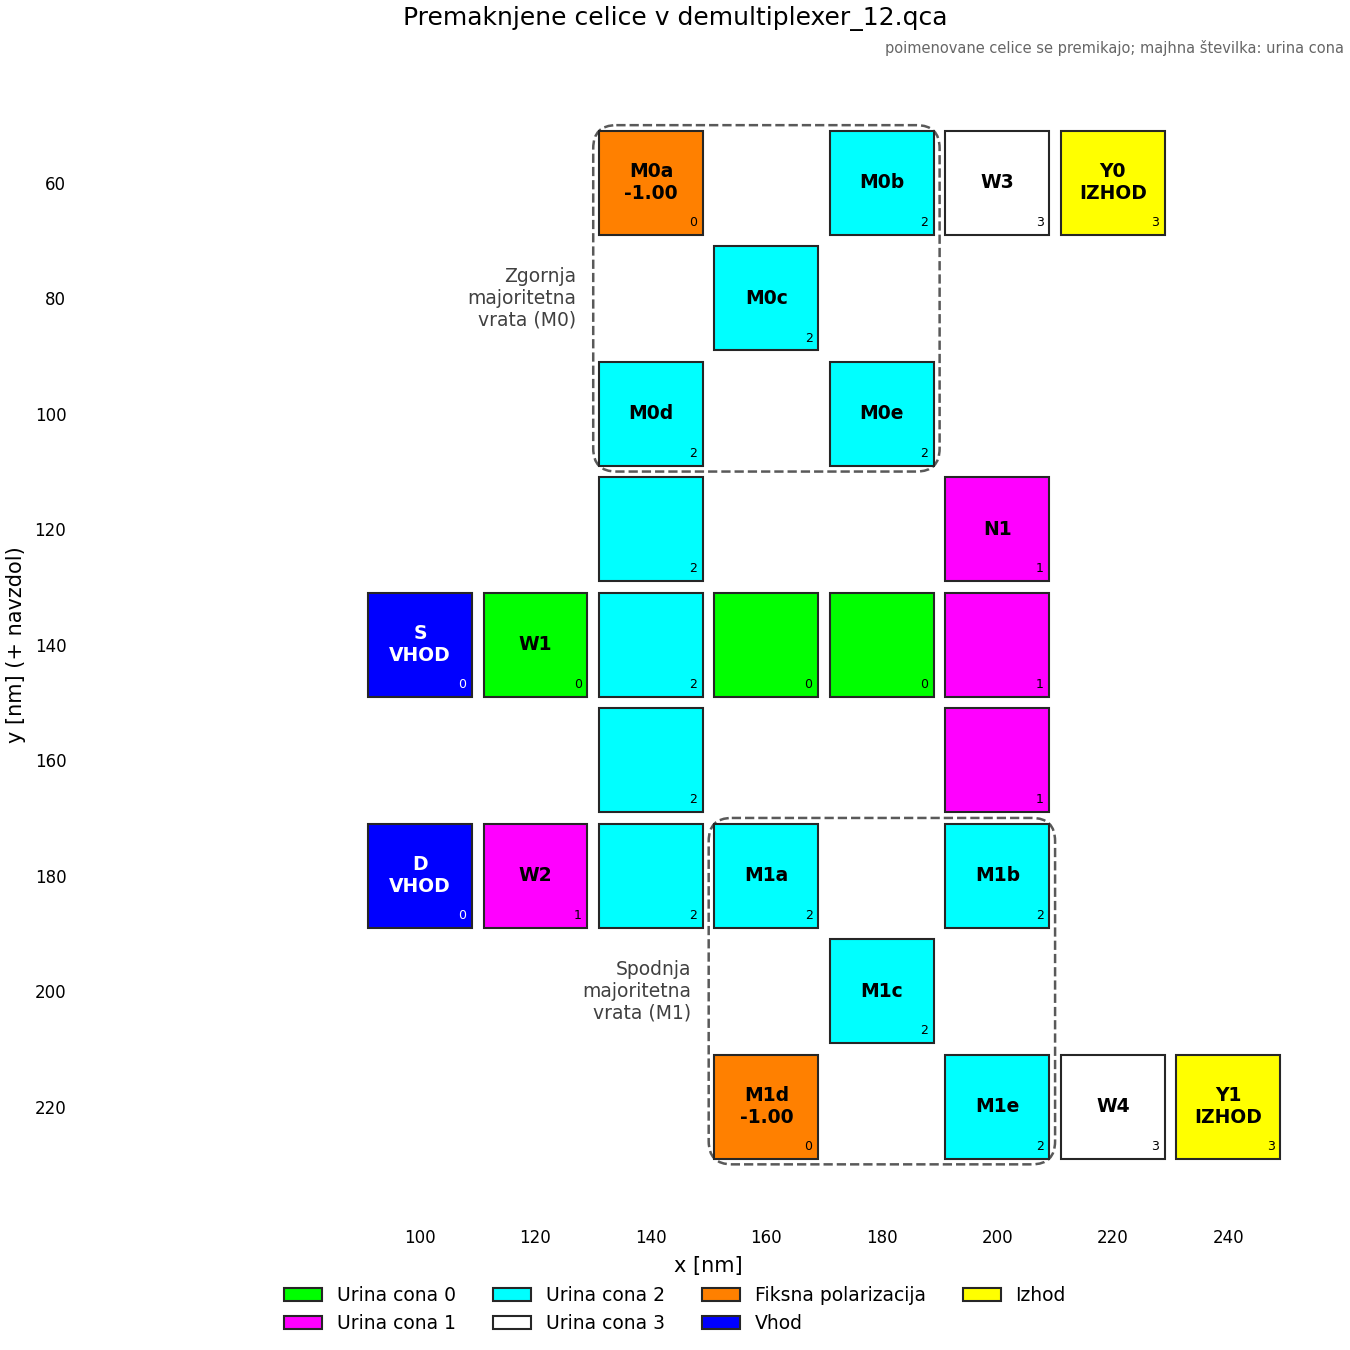
\includegraphics[width=0.9\textwidth]{cell-layout}
\caption{
    Shema demultiplekserja. 
    Celice so označene z imeni, ki so uporabljene za skicevanje nanje v nadaljevanju.
}
\label{g27:fig:shema}
\end{figure}

% NAŠA HIPOTEZA!!!
Predpostavljamo, da občutljivost vezja na premike celic ni enakomerna. Premiki celic v bližini logičnih vrat (NOT in majoritetnih vrat) bodo povzročili večje spremembe izhodne polarizacije in hitreje privedli do nepravilnega delovanja kot primerljivi premiki celic v ravnih povezovalnih vodilih.

Pričakujemo tudi, da bodo večji premiki povzročili izrazitejše odstopanje od rezultatov izvirne implementacije.
%%%%%%%%%%%%%%%%%%%%%%%

% [Opišite, katere poskuse ste izvedli in zakaj. Enačbe pišite v okolju \texttt{equation} in se nanje sklicujte, npr.\ polarizacija celice je določena z enačbo~\eqref{g27:eq:polarizacija}.]

% \begin{equation}
% P = \frac{(\rho_1 + \rho_3) - (\rho_2 + \rho_4)}{\rho_1 + \rho_2 + \rho_3 + \rho_4}
% \label{g27:eq:polarizacija}
% \end{equation}

% [Za izris kvantnih vezij lahko uporabite paket \texttt{quantikz}. Slika~\ref{g27:fig:bell} je primer vezja, ki pripravi Bellovo stanje $\frac{1}{\sqrt{2}}(\ket{00} + \ket{11})$.]

% \begin{figure}[htbp]
% \centering
% \begin{quantikz}
% \lstick{$\ket{0}$} & \gate{H} & \ctrl{1} & \meter{} \\
% \lstick{$\ket{0}$} & \qw      & \targ{}  & \meter{}
% \end{quantikz}
% \caption{Primer kvantnega vezja: priprava in merjenje Bellovega stanja.}
% \label{g27:fig:bell}
% \end{figure}

% [Kratke odseke kode lahko vključite z okoljem \texttt{lstlisting}, celotno kodo pa hranite v repozitoriju.]

% \begin{lstlisting}[language=Python, caption={Primer: izvedba vezja na kvantnem procesorju IBM.}, label={g27:lst:qiskit}]
% from qiskit import QuantumCircuit
% from qiskit.transpiler import generate_preset_pass_manager
% from qiskit_ibm_runtime import QiskitRuntimeService, SamplerV2 as Sampler
% 
% qc = QuantumCircuit(2)
% qc.h(0)
% qc.cx(0, 1)
% qc.measure_all()
% 
% backend = QiskitRuntimeService().least_busy(operational=True, simulator=False)
% isa = generate_preset_pass_manager(backend=backend, optimization_level=1).run(qc)
% job = Sampler(mode=backend).run([isa], shots=1000)
% print(job.job_id(), job.result()[0].data.meas.get_counts())
% \end{lstlisting}

%%%%%%%%%%%%%%%%%%%%%%%%%%%%%%
\subsection{Metrike}
\label{g27:sec:metrike}

Pri poskusu smo merili sledeče metrike, s katerimi smo ocenjevali robustnost demultiplekserja pri zamiku posameznih celic. 
\begin{enumerate}
    \item \textbf{Pravilnost izhoda} -- splošen pregled: pri katerih premikih demultiplekser pri istih vhodnih podatkih ohrani isti izhod. 
    \item \textbf{Toleranca na premik} -- koliko se lahko celica na določenem mestu premakne, da demultiplekser še vedno ohrani pravilen izhod.
    \item \textbf{Zanesljivost delovanja pri določenem premiku} -- kako zanesljivo bo v povprečju demultiplekser deloval, če eno celico zamaknemo za določeno razdaljo.
    \item \textbf{Velikost in stabilnost polarizacije} -- kakšno polarizacijo imajo izhodne celice v ustreznih fazah urinega cikla.
\end{enumerate}

Vse metrike bomo primerjali glede na izhode pri osnovnem modelu demultiplekserja s slike~\ref{g27:fig:shema}.

\section{Rezultati}
\label{g27:sec:rezultati}

\subsection{Pravilnost izhoda}
\label{g27:sec:pravilnost-izhoda}

Kot pričakovano, premiki celic za nekaj nanometrov v različnih smereh vplivajo na pravilno delovanje QCA demultiplekserja.
Pri različnih delih vezja imajo premiki različen vpliv. 
Tudi smer premika vpliva na pravilnost delovanja vezja. 
Iz Grafa~\ref{g27:fig:pravilnost-izhoda} lahko razberemo nekaj trendov: 

\begin{itemize}
    \item Najbolj občutljivo vodilo je vodilo W2, ko povezuje vhod D z demultiplekserjem.
    \item Zanimivo je, da sta si celici W1 in W2 različni v robustnosti, saj opravljata podobno funkcijo.
    Razlika se zelo verjetno pojavi zaradi interference med celicama, saj se lahko takšen vpliv prenaša samo v smeri naraščajoče ure, ne pa tudi v drugo smer.
    \item Negator je odporen na vse premike do \SI{5}{\nano\metre}.
    \item Majoritetna vrata 0 so veliko bolj občutljiva na premike kot majoritetna vrata 1.
    Takšno obnašanje bi lahko razložili s tem, da majoritetna vrata 0 prejmejo na vhodih veliko šibkejši signal, ki je prepotoval veliko daljšo pot, zato premiki celic veliko bolj vplivajo na izhod.
    \item V splošnem lahko opazimo, da na pravilnost delovanja najbolj vplivajo fiksno polarizirane celice (M0a in M1d) ter celice v sredini majoritetnih vrat (M0c in M1c).
    \item Šibkejši signal na M0 bi lahko tudi razložil razlike med celicama W3 in W4, saj celica W3 prejme šibkejši signal in zato na izhod Y0 premiki bolj vplivajo.
\end{itemize}


\begin{figure}[htbp]
    \centering
    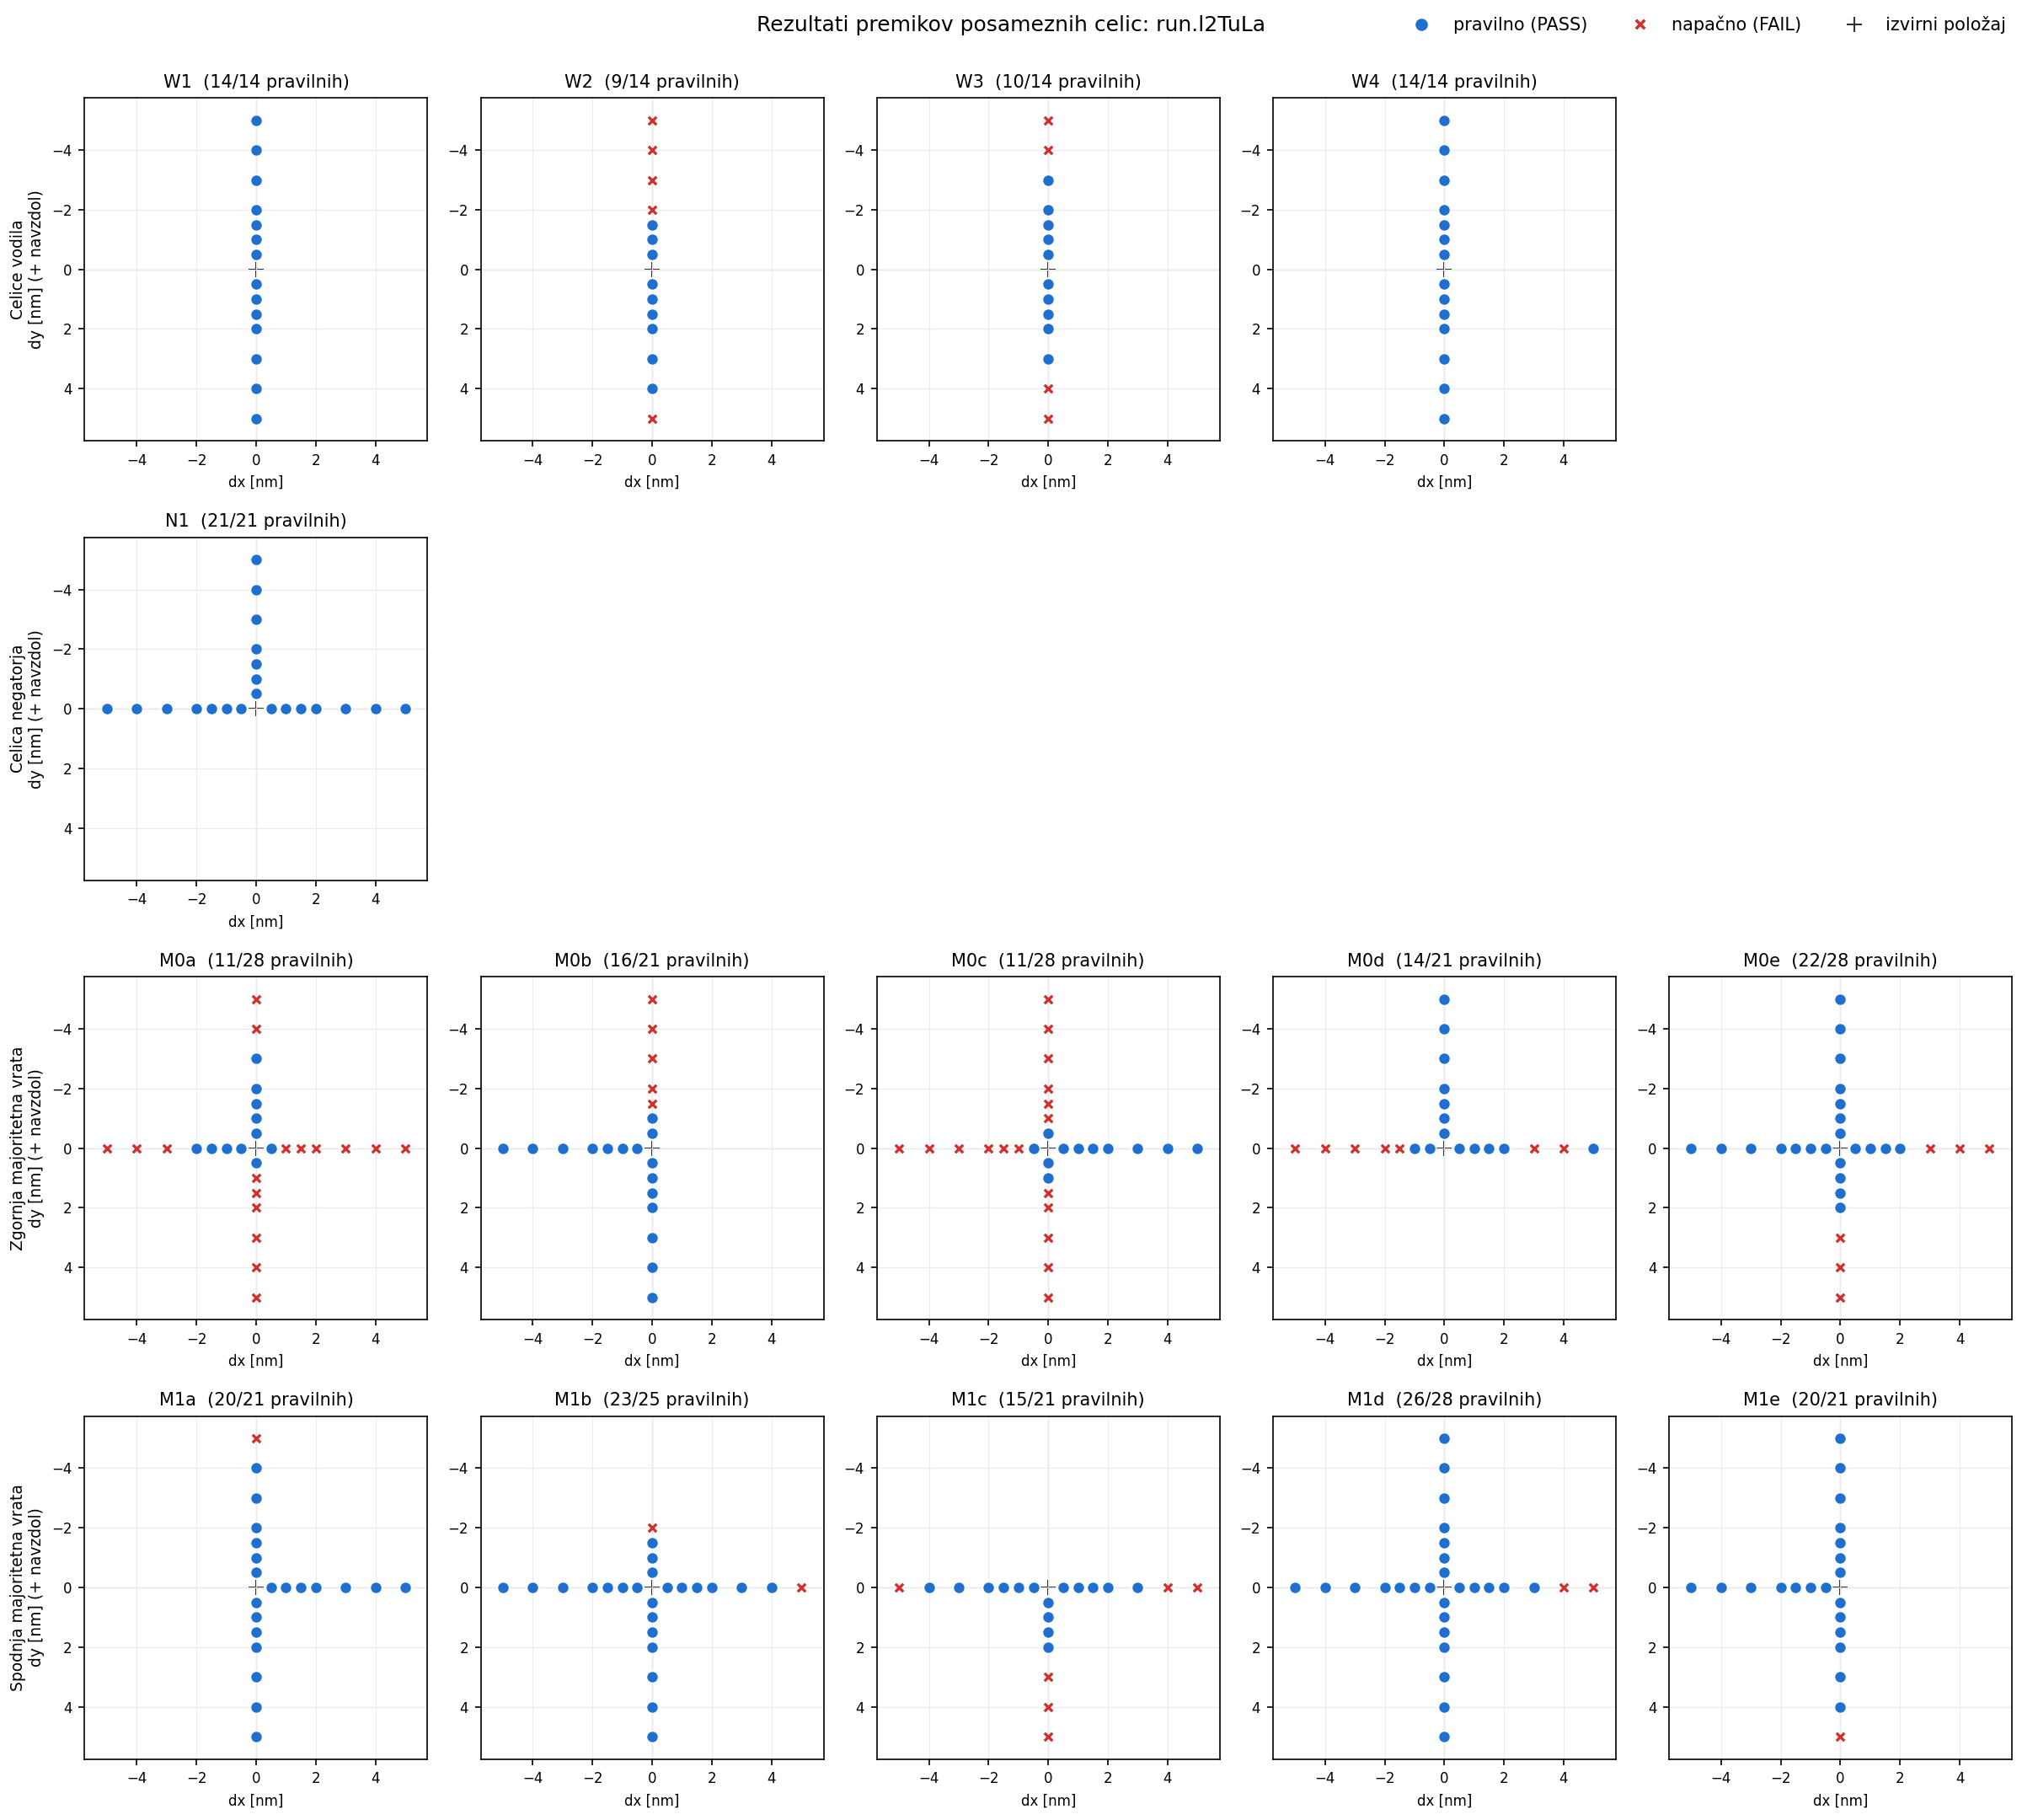
\includegraphics[width=1\textwidth]{displacement-overview}
    \caption{
        Pravilnost izhodov pri premikanju posmeznih celic demultiplekserja. 
        Vsaka vrstica prikazuje en del demultiplekserja (vodilo, negator, majoritetna vrata 0 in 1, od zgoraj navzdol). 
        Modre pike prikazujejo poskuse z uspešnim izhodom, rdeči križci pa tiste z neuspešnim. 
    }
    \label{g27:fig:pravilnost-izhoda}
\end{figure}
    
Imena celic, na katera se sklicujemo, so predstavlena na Sliki~\ref{g27:fig:shema}.


\subsection{Toleranca na premik}

Toleranco posamezne celice na premik smo ocenili kot povprečje razdalj, pri katerih celica v posamezni dovoljeni smeri prvič povzroči napačen izhod (Tabela~\ref{g27:tab:toleranca}).
Smeri, v katerih celica do največjega preizkušenega premika (\SI{5}{\nano\metre}) ni povzročila napake, smo v povprečje šteli s \SI{5}{\nano\metre}; v tem primeru je povprečje le spodnja meja prave tolerance in je označeno z $\geq$.

\begin{table}[htbp]
\centering
\small
\caption{
    Razdalja premika (v \si{\nano\metre}), pri kateri celica v posamezni smeri prvič povzroči napačen izhod, in njihovo povprečje.
    Oznaka $>5$ pomeni, da celica v tej smeri do \SI{5}{\nano\metre} ni povzročila napake, \enquote{--} pa, da premik v tej smeri ni bil dovoljen.
}
\label{g27:tab:toleranca}
\begin{tabular}{lccccc}
\toprule
Celica & $+x$ (desno) & $-x$ (levo) & $+y$ (dol) & $-y$ (gor) & Povprečje \\
\midrule
W1  & --    & --    & $>5$  & $>5$  & $\geq$\,5,00 \\
W2  & --    & --    & 5     & 2     & 3,50 \\
W3  & --    & --    & 4     & 4     & 4,00 \\
W4  & --    & --    & $>5$  & $>5$  & $\geq$\,5,00 \\
\midrule
N1  & $>5$  & $>5$  & --    & $>5$  & $\geq$\,5,00 \\
\midrule
M0a & 1     & 3     & 1     & 4     & 2,25 \\
M0b & --    & $>5$  & $>5$  & 1,5   & $\geq$\,3,83 \\
M0c & $>5$  & 1     & 1,5   & 1     & $\geq$\,2,13 \\
M0d & 3     & 1,5   & --    & $>5$  & $\geq$\,3,17 \\
M0e & 3     & $>5$  & 3     & $>5$  & $\geq$\,4,00 \\
\midrule
M1a & $>5$  & --    & $>5$  & 5     & $\geq$\,5,00 \\
M1b & 5     & $>5$  & $>5$  & 2     & $\geq$\,4,25 \\
M1c & 4     & 5     & 3     & --    & 4,00 \\
M1d & 4     & $>5$  & $>5$  & $>5$  & $\geq$\,4,75 \\
M1e & --    & $>5$  & 5     & $>5$  & $\geq$\,5,00 \\
\bottomrule
\end{tabular}
\end{table}

\subsection{Zanesljivost delovanja pri določenem premiku}

Kumulativni delež neuspešnih scenarijev po velikosti premika je prikazan na Sliki~\ref{g27:fig:kumulativno}. 
Trend naraščanja nepravilnih izhodov demultiplekserja s povečavanjem odmika od njihove načrtovane lege je očiten. 

\begin{figure}[htbp]
\centering
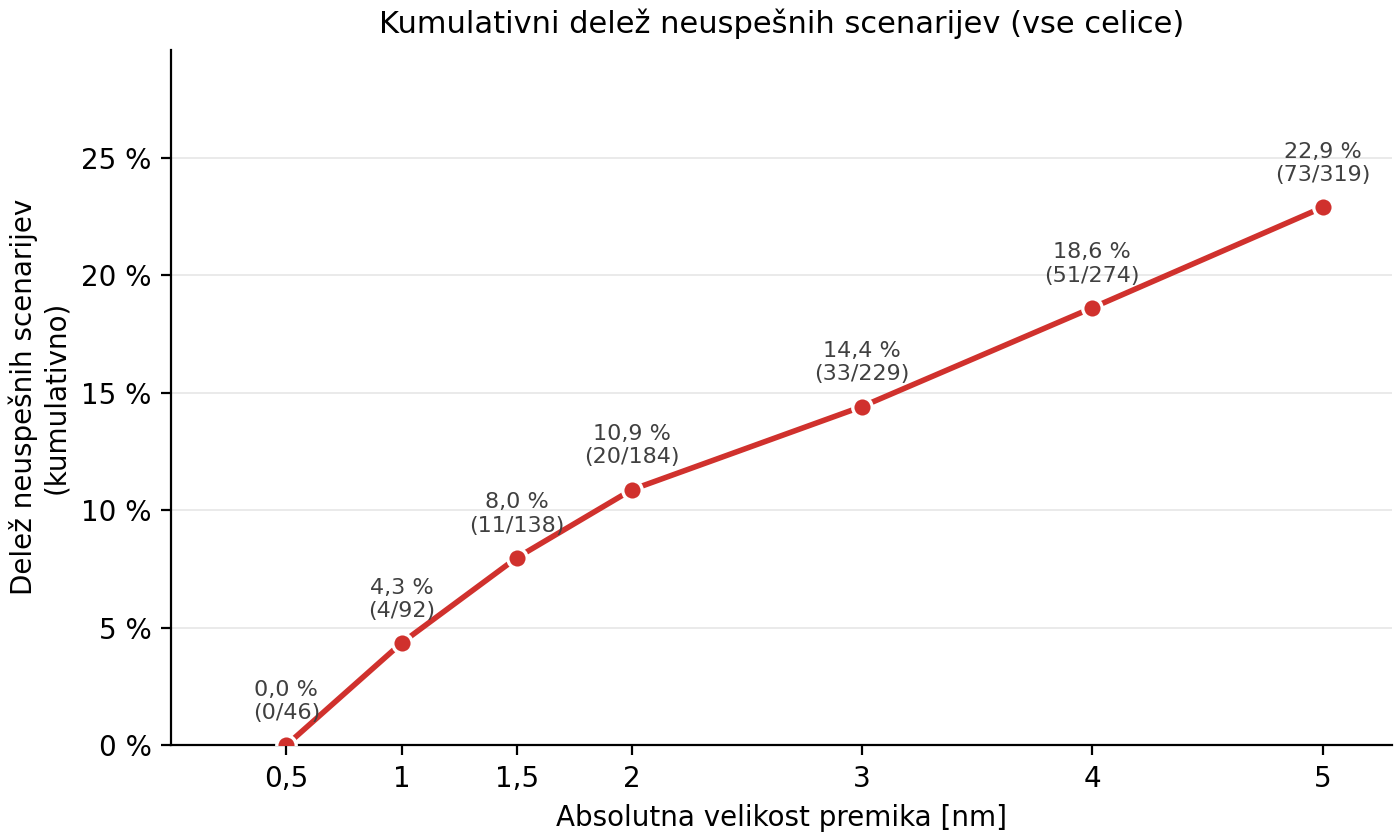
\includegraphics[width=0.75\textwidth]{cumulative-failures}
\caption{
    Kumulativni delež neuspešnih scenarijev glede na absolutno velikost premika, za vse celice in vse smeri skupaj.
    Pri vsakem odmiku je prikazan delež neuspešnih med vsemi poskusi s premikom, manjšim ali enakim temu odmiku; oznaka ob točki podaja še razmerje \emph{neuspešni/vsi}.
}
\label{g27:fig:kumulativno}
\end{figure}


\subsection{Velikost in stabilnost polarizacije}

Pri vsakem poskusu smo merili polarizacijo na izhodnih celicah, da bi ugotovili, kako močno določeni premiki vplivjo nanjo. 
Meritve izhodne polarizacije so prikazane za vse možne premike za Y0 na grafu~\ref{g27:fig:y0} ter za Y1 na grafu~\ref{g27:fig:y1}.
Iz grafov je jasno razvidno, da imajo na polarizacijo opazen vpliv samo premiki celic W3 in W4.
To sta celici, ki sta neposredna soseda izhodnih celic.

\begin{figure}[htbp]
\centering
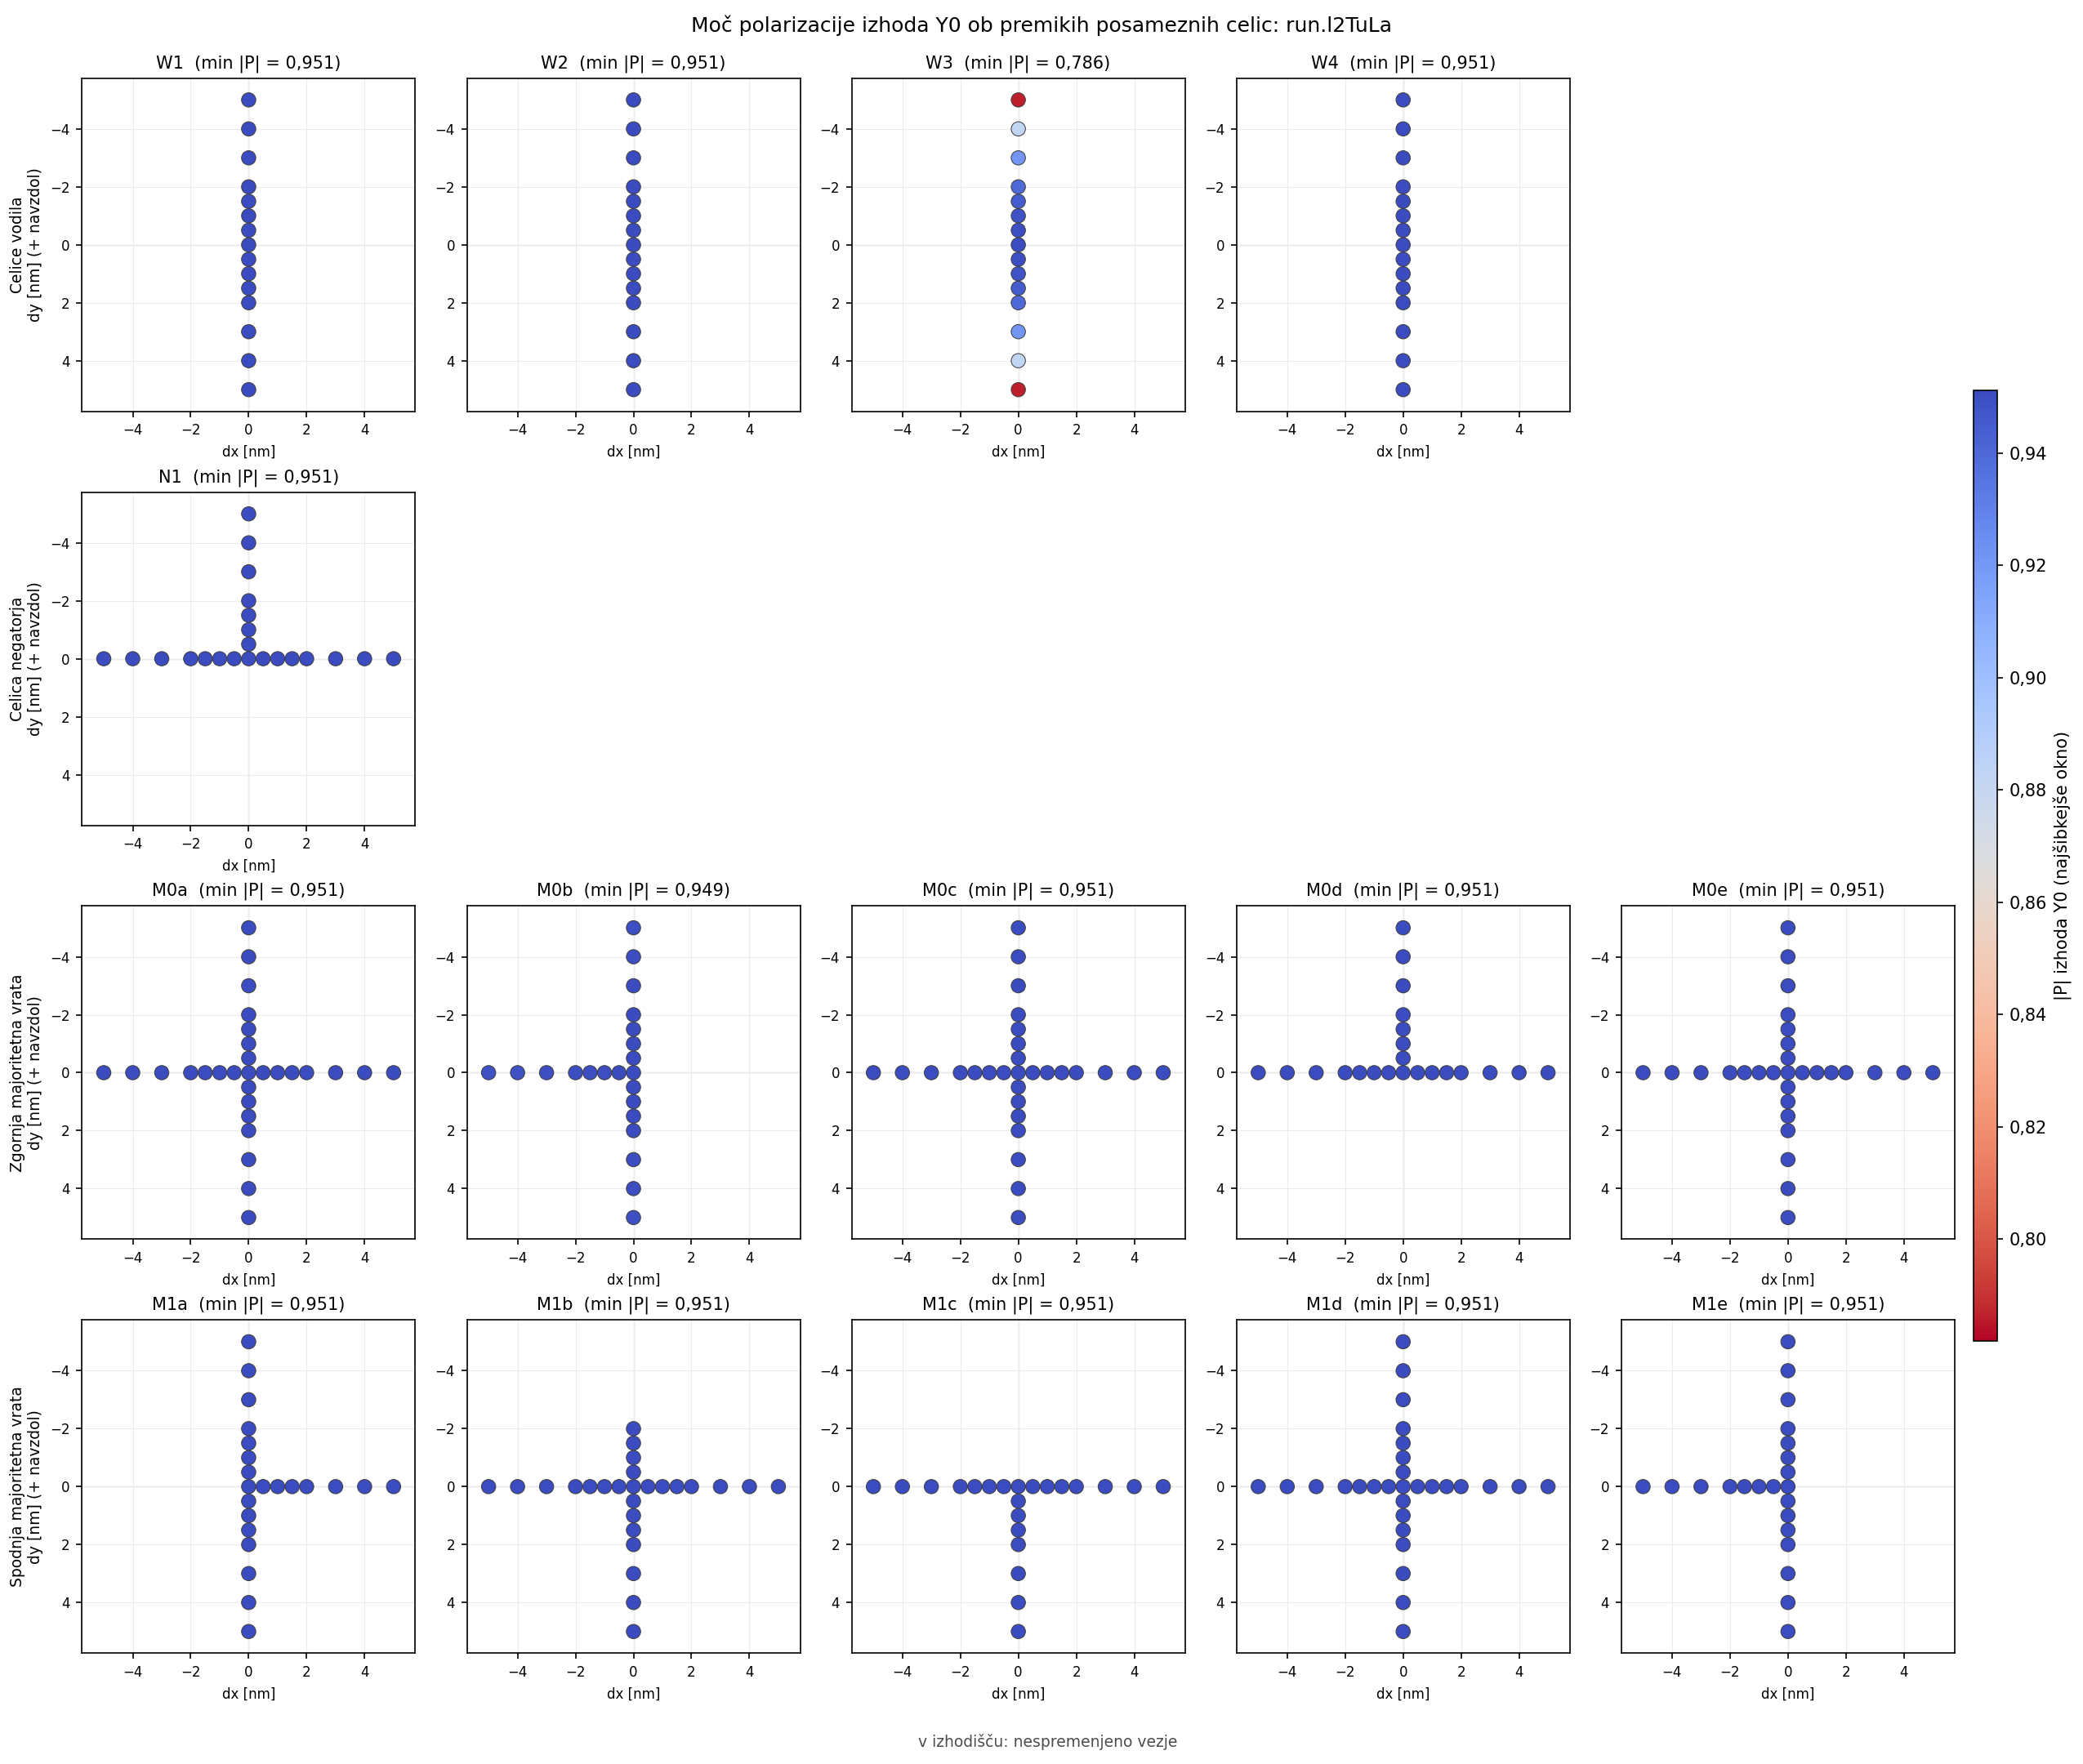
\includegraphics[width=1\textwidth]{polarization-Y0}
\caption{
    Polarizacija izhoda Y0. Polarizacija je prikazana za vse možne premike. 
    Absolutna vrednost polarizacije je prikazana s pomočjo barvne lestvice.
}
\label{g27:fig:y0}
\end{figure}


\begin{figure}[htbp]
\centering
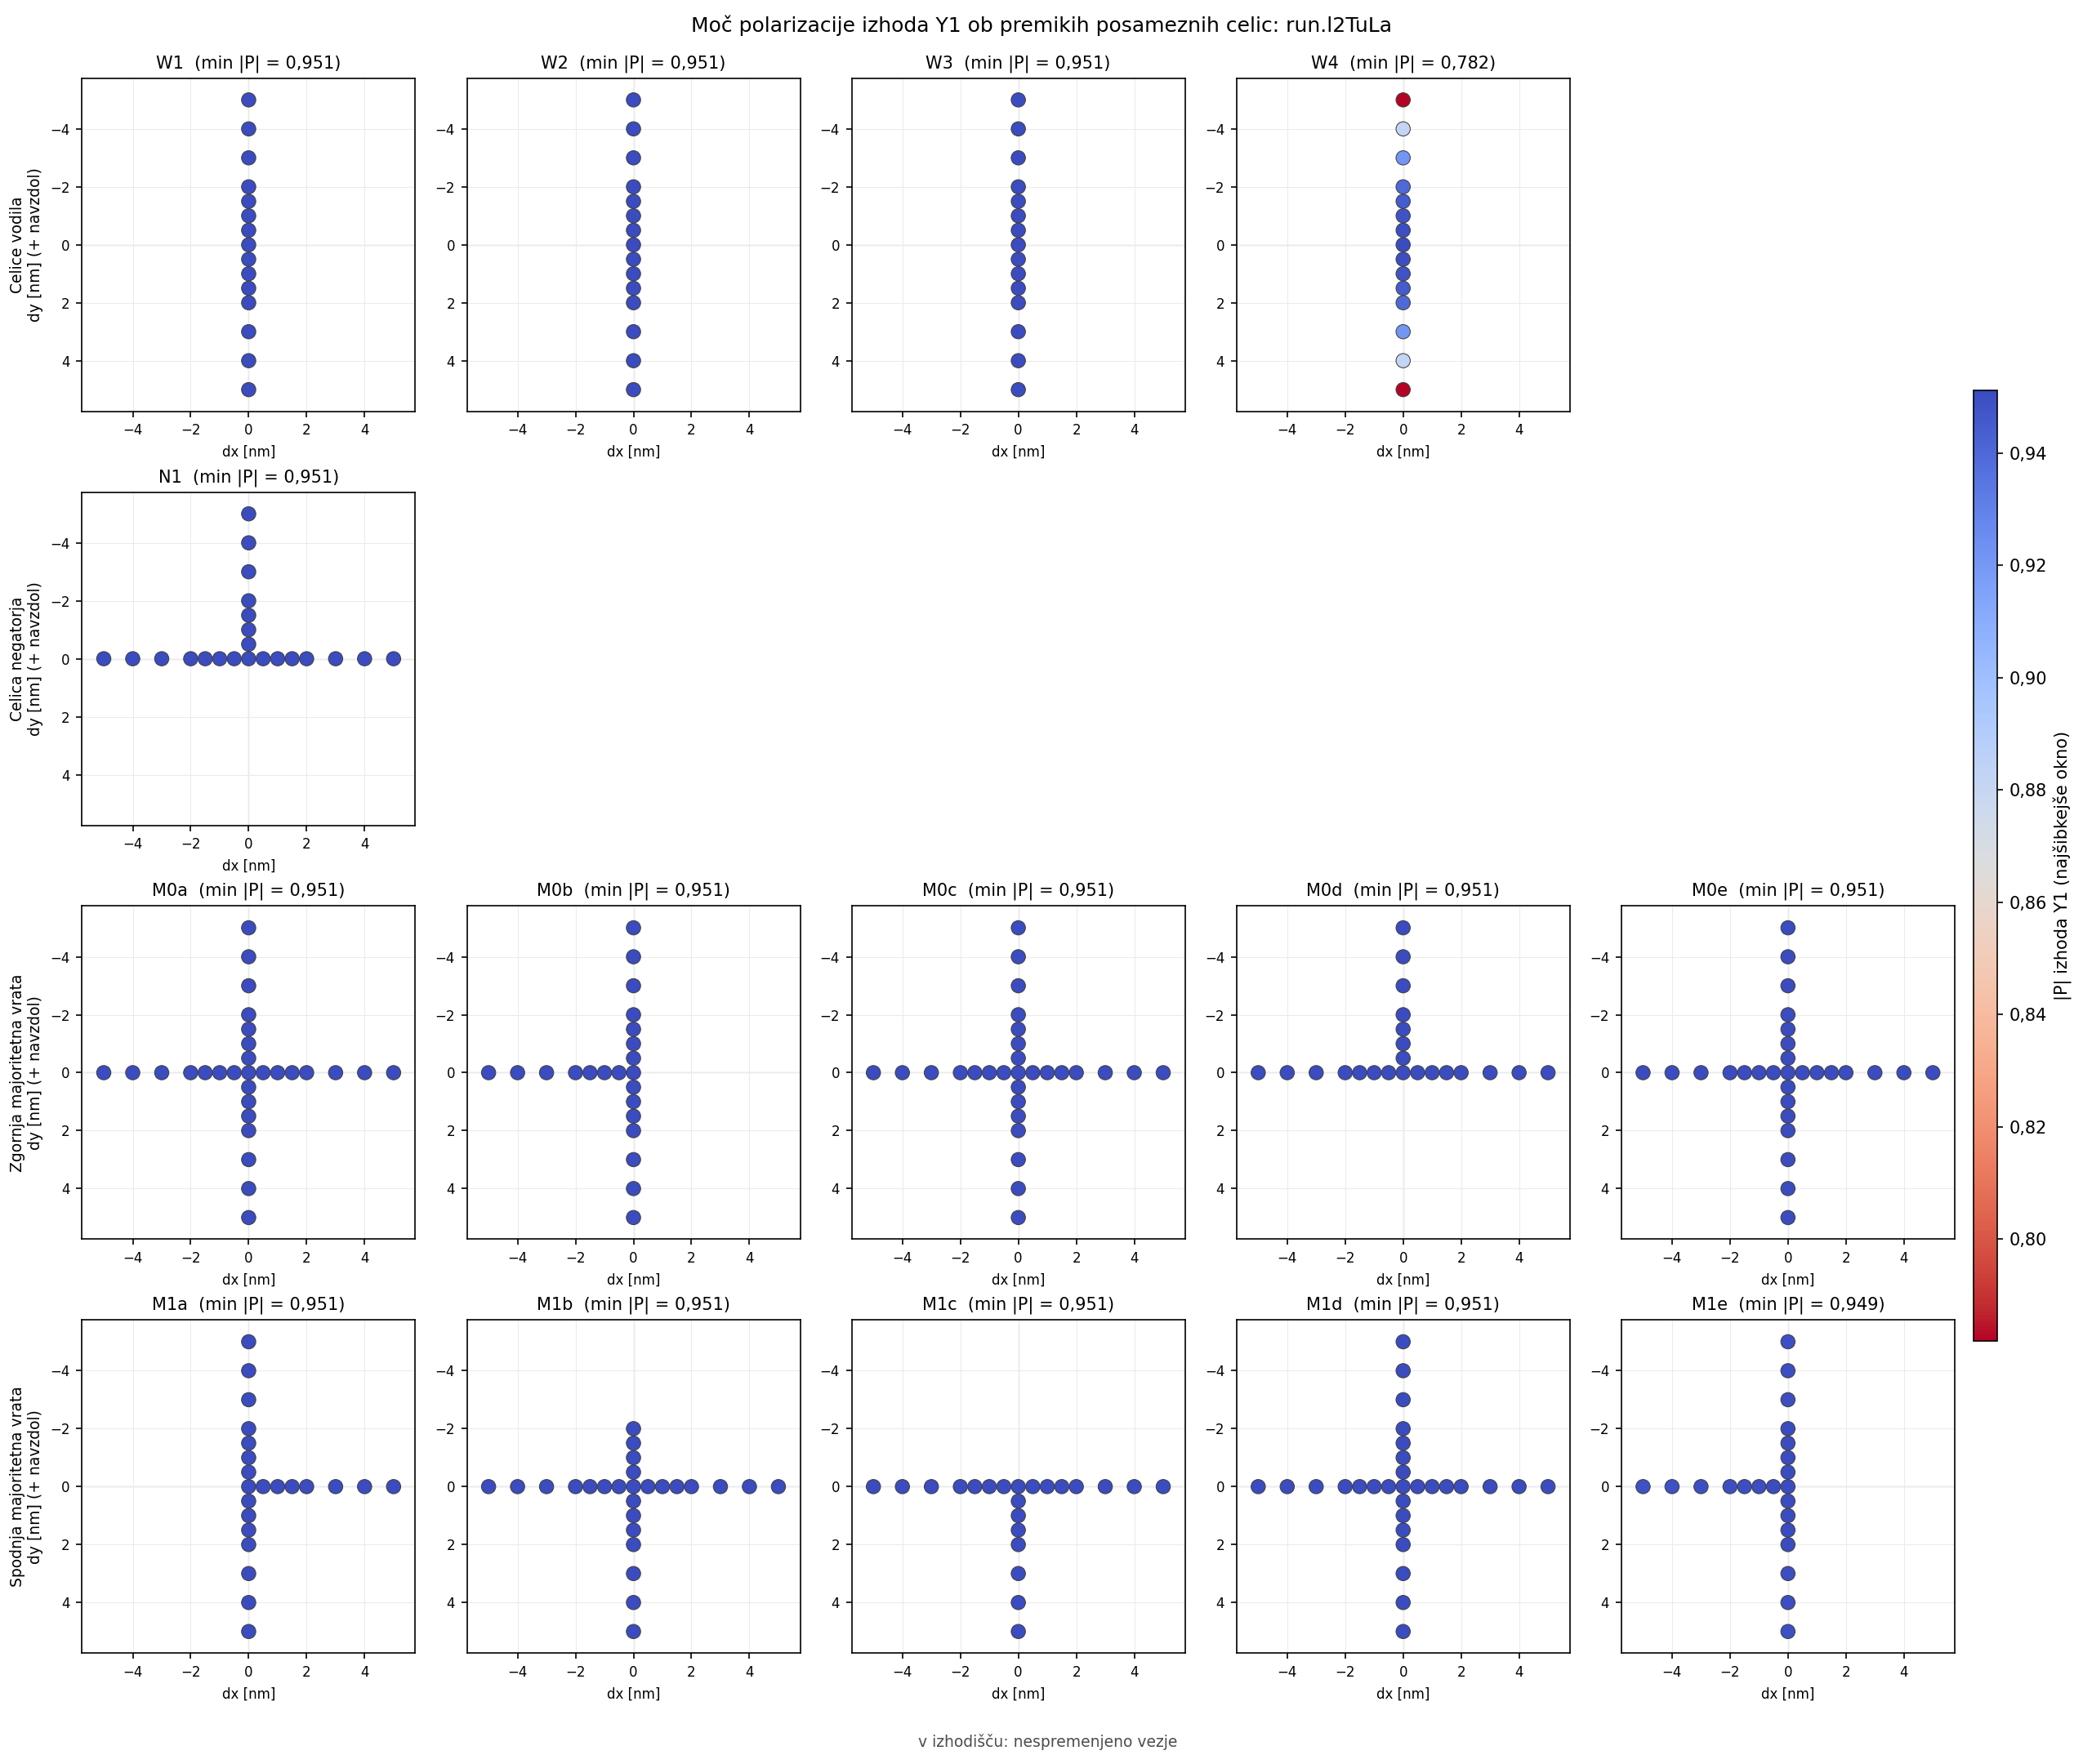
\includegraphics[width=1\textwidth]{polarization-Y1}
\caption{
    Polarizacija izhoda Y1. Polarizacija je prikazana za vse možne premike. 
    Absolutna vrednost polarizacije je prikazana s pomočjo barvne lestvice.
}
\label{g27:fig:y1}
\end{figure}


%%%%%%%%%%%%%%%%%%%%%%%%


\section{Razprava}

\label{g27:sec:razprava}
% [Odgovorite na raziskovalno vprašanje in rezultat primerjajte s pričakovanim. Opišite omejitve: kaj vaši rezultati pokažejo in česa ne.]

Rezultati simulacij potrjujejo, da je delovanje QCA-demultiplekserja občutljivo na fizične premike posameznih celic. Vpliv premikov ni enakomerno porazdeljen po vezju, temveč je odvisen od položaja celice, smeri premika in vloge, ki jo celica opravlja. S tem smo potrdili začetno hipotezo, da so celice v območju logičnih vrat praviloma občutljivejše od celic v povezovalnih vodilih.

Največjo občutljivost smo opazili pri celicah majoritetnih vrat 0, predvsem pri celicah M0a in M0c. Njuna povprečna toleranca na premik znaša približno \SI{2,25}{\nano\metre} oziroma največ \SI{2,13}{\nano\metre}, pri čemer je slednja zaradi nekaterih smeri brez zaznane napake le spodnja meja dejanske tolerance. To kaže, da lahko že razmeroma majhni premiki bistveno vplivajo na pravilnost delovanja logičnih vrat. Ena izmed možnih razlag je šibkejša vhodna polarizacija, saj signali do teh vrat potujejo po daljši poti in so zato bolj izpostavljeni motnjam.

Zanimiva je tudi razlika med občutljivostjo majoritetnih vrat 0 in 1. Vrata 0 so se izkazala za občutno občutljivejša, kar podpira predpostavko, da je njihovo delovanje zaradi šibkejšega vhodnega signala manj robustno. Pri tem imajo pomembno vlogo tudi fiksno polarizirane celice, saj lahko njihovi premiki spremenijo pogoje, pod katerimi se določi izhodna polarizacija vrat.

Med povezovalnimi vodili je bila najbolj občutljiva celica W2, pri kateri je že premik za \SI{2}{\nano\metre} v eni smeri povzročil napačen izhod. Nasprotno sta bili celici W1 in W4 odporni na vse preizkušene premike do \SI{5}{\nano\metre}. Razlika med celicama W1 in W2 je posebej zanimiva, saj opravljata podobno funkcijo. Možna razlaga je vpliv sosednjih celic in časovnega zaporedja prenosa polarizacije, vendar bi bilo za potrditev te razlage potrebno izvesti dodatne simulacije.

Negator se je izkazal za najbolj robusten logični element, saj pri nobenem izmed preizkušenih premikov do \SI{5}{\nano\metre} ni povzročil napačnega izhoda. To kaže, da vsi logični elementi niso enako občutljivi na geometrijske nepravilnosti in da je odpornost odvisna tudi od njihove zasnove.

Analiza izhodne polarizacije je pokazala, da večina premikov nima opaznega neposrednega vpliva na polarizacijo izhodnih celic. Najizrazitejši vpliv sta imela premika celic W3 in W4, ki sta neposredni sosedi izhodnih celic. To je pričakovano, saj se informacija v QCA prenaša preko elektrostatičnih interakcij med sosednjimi celicami. Sprememba njune medsebojne razdalje zato neposredno vpliva na polarizacijo izhodov.

Rezultati kumulativne analize neuspešnih scenarijev dodatno potrjujejo, da se z večanjem premika povečuje verjetnost nepravilnega delovanja vezja. Pri tem pa sama velikost premika ni edini odločilni dejavnik, saj lahko tudi manjši premik na občutljivem mestu povzroči napako, medtem ko večji premik na manj občutljivem mestu nima opaznega vpliva.

Pri interpretaciji rezultatov je treba upoštevati tudi omejitve eksperimenta. Preizkušeno je bilo omejeno število celic, velikosti premikov in smeri. Poleg tega so bile simulacije izvedene za posamezne premike, medtem ko se lahko pri dejanski izdelavi pojavijo hkratna odstopanja več celic. Zato dobljenih rezultatov ne moremo neposredno posplošiti na vse možne implementacije QCA-vezij.



\subsection{Kaj ni delovalo}
\label{g27:sec:neuspehi}
% [Opišite vsaj en poskus, ki ni uspel, kaj ste opazili in zakaj po vašem mnenju ni deloval.]

Pri M0d demux ne deluje pri px=4, pri px=5 pa. To je neka anomalija, ki je ne znamo razložiti. 
+ Pričakovali smo, da bo polarizacija različna za različne tipe premikov, a je skoraj vedno enaka (torej popolnoma pravilna ali popolnoma napačna).

\section{Zaključek}
\label{g27:sec:zakljucek}

V projektu smo raziskali vpliv fizičnih premikov posameznih celic na delovanje QCA-demultiplekserja $1:2$, sestavljenega iz 27 celic. Z uporabo programa QCADesigner-E smo analizirali pravilnost izhodov, toleranco posameznih celic na premike ter vpliv premikov na izhodno polarizacijo.

Rezultati so pokazali, da občutljivost na premike ni enakomerno porazdeljena po vezju. Najbolj občutljive so se izkazale celice v majoritetnih vratih 0, predvsem M0a in M0c, ter celica W2 na vhodnem povezovalnem vodilu. Nasprotno se je negator izkazal za zelo robustnega, saj preizkušeni premiki do \SI{5}{\nano\metre} niso povzročili nepravilnega delovanja. Potrdili smo tudi, da na občutljivost vplivata smer in velikost premika.

Analiza polarizacije je pokazala, da imajo na izhodne celice največji neposredni vpliv premiki njihovih sosednjih celic W3 in W4. Poleg tega smo ugotovili, da se z večanjem velikosti premikov povečuje delež neuspešnih simulacij.

Na podlagi rezultatov lahko sklenemo, da je pri načrtovanju QCA-vezij poleg števila celic, velikosti in zakasnitve pomembno upoštevati tudi njihovo odpornost na fizična odstopanja. Ugotovitve kažejo, da je smiselno posebno pozornost nameniti celicam v majoritetnih vratih in tistim, ki neposredno vplivajo na prenos informacij med posameznimi deli vezja.

\subsection{Nadaljnje delo}
% [Povzemite glavni rezultat v nekaj stavkih in predlagajte, kako bi delo nadaljevali.]

Raziskavo bi bilo mogoče razširiti v več smereh. Najprej bi bilo smiselno preveriti večje premike celic, predvsem na mestih, kjer pri dosedanjih simulacijah napak še nismo zaznali. Tako bi lahko natančneje določili meje tolerance posameznih celic.

Pomembna razširitev bi bila tudi analiza hkratnih premikov več celic. V tem projektu smo namreč premikali posamezne celice, medtem ko lahko pri dejanski izdelavi vezja pride do odstopanj na več mestih hkrati. Takšni premiki bi se lahko medsebojno krepili ali izničili.

Poleg tega bi bilo zanimivo raziskati vpliv različnih vrst napak, kot so manjkajoče celice, spremembe dimenzij celic in napake pri njihovi orientaciji. Raziskavo bi lahko razširili tudi na druge implementacije demultiplekserjev ter primerjali njihovo odpornost na enake motnje.

Nazadnje bi bilo smiselno podrobneje analizirati energijsko disipacijo in časovni potek polarizacije pri najbolj občutljivih celicah. S tem bi lahko bolje razumeli, kako fizični premiki vplivajo na stabilnost prenosa informacij in energijsko učinkovitost QCA-vezij.


\section*{Doprinosi avtorjev}

% [Za vsakega člana v dveh do treh stavkih: kateri del izdelka in poročila je pripravil. Npr.\ \enquote{Ime Priimek je zasnoval in simuliral reverzibilni seštevalnik, pripravil sliko~\ref{g27:fig:majoritetna} in napisal poglavje~\ref{g27:sec:metode}.}]
Matic Poženel je pripravil implementacijo demultiplekserja v QCADesignerju in orodja za testiranje konfiguracij implementacije.\\
\noindent
Vojko Hysz je testiral vezje z različnimi konfiguracijami in napisal poglavje~\ref{g27:sec:rezultati}.\\
\noindent
Gašper Suhadolnik je napisal poglavja~\ref{g27:sec:uvod}, \ref{g27:sec:metode}, \ref{g27:sec:razprava}, \ref{g27:sec:zakljucek} in oblikoval poročilo.\\

\section*{Izjava o uporabi generativne umetne inteligence}

% TODO - bolj natančno?
% [Navedite orodja in za kaj ste jih uporabili. Npr. pomoč pri pisanju kode, lektoriranje ali iskanje virov. Če orodij niste uporabili, to zapišite.]
Pri izdelavi seminarske naloge smo uporabljali orodja umetne inteligence pri pisanju kode, lektoriranju besedila in iskanju virov.
